\documentclass[10pt,a4paper]{article}
\usepackage[margin=18mm]{geometry}
\usepackage[T1]{fontenc}
\usepackage{helvet}\renewcommand{\familydefault}{\sfdefault}
\usepackage{graphicx,booktabs,xcolor,tikz,enumitem,amsmath,array}
\usepackage[hidelinks]{hyperref}
\definecolor{acc}{HTML}{2F5D9E}\definecolor{iron}{HTML}{9A4A2A}\definecolor{he}{HTML}{1F7F78}\definecolor{mut}{HTML}{5B6577}\definecolor{warn}{HTML}{A86A00}
\setlist{nosep,leftmargin=1.2em}
\newcommand{\sect}[1]{\par\medskip{\large\bfseries\color{acc}#1}\par\smallskip}
\newcommand{\boxit}[2]{\par\noindent\fcolorbox{#1}{#1!6}{\parbox{\dimexpr\linewidth-2\fboxsep-2\fboxrule}{#2}}\par}
\pagestyle{plain}
\begin{document}
{\small\color{mut}SHiP veto $\cdot$ fastveto + shield\_dis $\cdot$ branch veto-shield-dis $\cdot$ 3 Nov 2026}\\[2pt]
{\LARGE\bfseries How the muon DIS chain works}\par\medskip
There are two chains that share one engine. The \textbf{\color{he}vessel chain} forces $\mu$--nucleus interactions in the helium, air, PVC walls and veto planes ($z = 30.6$--$82$\,m). The \textbf{\color{iron}shield chain} forces them in the last 50\,cm of MS7 iron and adds a Geant4 transport out of the iron. Both chains then go through the same selection and veto code.

\sect{1 \quad Where the interactions happen}
\begin{center}
\resizebox{\linewidth}{!}{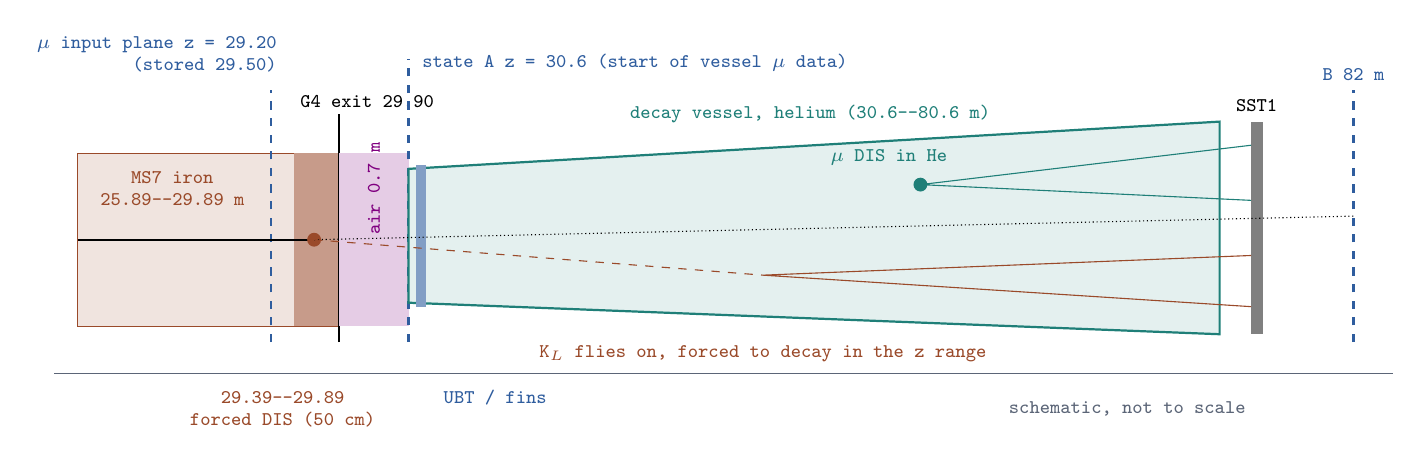
\begin{tikzpicture}[x=1cm,y=1cm,font=\scriptsize\ttfamily]
\draw[mut] (0,0)--(17,0);
\fill[iron!15] (0.3,0.6) rectangle (3.6,2.8); \draw[iron] (0.3,0.6) rectangle (3.6,2.8);
\node[iron,align=center] at (1.5,2.35) {MS7 iron\\25.89--29.89 m};
\fill[iron!55] (3.05,0.6) rectangle (3.6,2.8);
\node[iron,align=center] at (2.9,-0.45) {29.39--29.89\\forced DIS (50 cm)};
\draw[acc,dashed,thick] (2.75,0.4)--(2.75,3.6); \node[acc,anchor=east,align=right] at (2.95,4.05) {$\mu$ input plane z = 29.20\\(stored 29.50)};
\draw[thick] (3.62,0.4)--(3.62,3.3); \node[anchor=west] at (3.0,3.45) {G4 exit 29.90};
\fill[violet!20] (3.62,0.6) rectangle (4.5,2.8); \node[violet,rotate=90] at (4.06,2.35) {air 0.7 m};
\draw[acc,dashed,thick] (4.5,0.4)--(4.5,4.0); \node[acc,anchor=west] at (4.55,3.95) {state A z = 30.6 (start of vessel $\mu$ data)};
\fill[he!12] (4.5,0.9)--(14.8,0.5)--(14.8,3.2)--(4.5,2.6)--cycle; \draw[he,thick] (4.5,0.9)--(14.8,0.5)--(14.8,3.2)--(4.5,2.6)--cycle;
\node[he] at (9.6,3.3) {decay vessel, helium (30.6--80.6 m)};
\fill[acc!60] (4.6,0.85) rectangle (4.72,2.65); \node[acc] at (5.6,-0.3) {UBT / fins};
\fill[black!50] (15.2,0.5) rectangle (15.35,3.2); \node at (15.27,3.4) {SST1};
\draw[acc,dashed,thick] (16.5,0.4)--(16.5,3.6); \node[acc] at (16.5,3.8) {B 82 m};
\draw[thick] (0.3,1.7)--(3.3,1.7); \fill[iron] (3.3,1.7) circle (2.5pt);
\draw[densely dotted] (3.3,1.7)--(16.5,2.0);
\draw[iron,dashed] (3.3,1.7)--(9.0,1.25); \draw[iron] (9.0,1.25)--(15.2,0.85) (9.0,1.25)--(15.2,1.5);
\node[iron] at (9.0,0.25) {K$_L$ flies on, forced to decay in the z range};
\fill[he] (11,2.4) circle (2.5pt); \draw[he] (11,2.4)--(15.2,2.9) (11,2.4)--(15.2,2.2);
\node[he] at (10.6,2.75) {$\mu$ DIS in He};
\node[mut,anchor=west] at (12,-0.45) {schematic, not to scale};
\end{tikzpicture}}
\end{center}

\sect{2 \quad The whole chain at a glance}
\begin{center}\includegraphics[height=0.55\textheight]{overview.pdf}\end{center}

\newpage
\sect{3 \quad Forced interactions and weights}
DIS is rare ($P\approx10^{-3}$ for 50\,cm of iron, far less in helium), so each interaction is forced and the probability goes into the weight. Draws are importance-sampled per target group (helium, air, PVC, each plane, shield iron).
\begin{align*}
P_i &= n_{\text{area}}\,\sigma(E_i), \qquad n_{\text{area}} = \text{nucleons per m}^2\text{ along the chord}\\
S_g &= \textstyle\sum_{i\in g} w_i P_i \qquad \text{(interactions per spill in group } g)\\
\text{``}M\text{ draws'':}&\ \ \text{pick crossing } i \text{ with prob. } w_iP_i/S_g, \quad \text{weight } S_g/M \text{ each}\\
\text{``per track'' (draws}=-k):&\ \ k \text{ draws on every crossing}, \quad \text{weight } w_iP_i/k \text{ each}\\
\text{per 15 years} &= \text{weight}\times 6\times10^{20}/5\times10^{13}\ \text{spills}
\end{align*}
\begin{itemize}
\item \textbf{$M$ draws $\propto w P$ (default):} spends the MC where the rate is. A few high-weight input muons can dominate (the 768.75 class is about 40\,\% of the shield DIS rate).
\item \textbf{One per crossing/track:} every parent contributes once. Same central values; the $\mu$ errors stay because they come from the few independent input muons (evt\_n), not from the number of draws.
\end{itemize}

\sect{4 \quad The interaction library (bin/dis\_library.py)}
\begin{center}\includegraphics[width=\linewidth]{library.pdf}\end{center}
\begin{itemize}
\item $\sigma$ per nucleon of each part = generator $\sigma$ $\times$ the fraction of its events on that side of $\nu_x$. Iron is $0.82\times$ helium per nucleon (Kokoulin shadowing). The Pythia share is 1.5\,\% at 10\,GeV and 13\,\% at 100\,GeV.
\item Only $\mu^-$ is generated. With one-photon exchange the hadronic final state is the same for $\mu^+$, so only the beam-muon sign is flipped.
\item Sampling: one of the two neighbouring grid energies (linear in $\log E$, no rescaling), event rotated to the muon direction with a random azimuth.
\item By default K$_S$, $\Lambda$, $\Sigma$, $\Xi$, $\Omega$, $\pi^0$ and $\eta$ are decayed at generation. That is right in helium but wrong in iron, so the \texttt{--stable-v0} library keeps K$_S$ and $\Lambda$ for Geant4 to absorb or decay in flight.
\item Neutrino version: GENIE 3.06.02 G18\_02a (Fe56 for the shield), using the same draw logic (\texttt{fastveto.nudis}).
\end{itemize}

\sect{5 \quad What differs between the two chains}
\noindent\begin{tabular}{@{}>{\raggedright\arraybackslash}p{0.48\linewidth}@{\hspace{0.04\linewidth}}>{\raggedright\arraybackslash}p{0.48\linewidth}@{}}
\textbf{\color{he}Vessel chain} \texttt{fastveto.dis.run} & \textbf{\color{iron}Shield chain} \texttt{bin/shield\_dis.py}\\[2pt]
\begin{itemize}
\item Targets: helium (code 0), air (1), PVC (2), plane $i$ (10+$i$)
\item Muon path A$\to$(K)$\to$B; $E$ interpolated in $z$
\item Planes: slab of the technology's material, thickness$/|\cos\theta|$ (cap 0.02)
\item Products are straight lines (no field before the spectrometer)
\item The scattered $\mu$ keeps its parent's upstream hits, so the veto can see the parent
\item \texttt{bin/run\_interactions.py --design D}
\end{itemize}
&
\begin{itemize}
\item Target: iron box; codes 3 (interaction) and 4 (V0-decay copy)
\item Straight parents from 29.20\,m; muons that stop in the slab not removed (mean loss only)
\item Geant4 transport of every product: absorption and cascade included, so no extra $e^{-d/\lambda}$ weight
\item Forced V0 decay copies (Sec.~7)
\item \texttt{beam = False}: no parent hits upstream
\item \texttt{prepare} $\to$ \texttt{g4.sh \dots\ generate} $\to$ \texttt{run\_interactions.py --interactions}
\end{itemize}
\end{tabular}

\newpage
\sect{6 \quad Shield chain step by step}
\begin{center}\includegraphics[width=\linewidth]{shield.pdf}\end{center}
{\small\color{mut}Per spill (= Hz at $5\times10^{13}$ PoT/s), $p>1$\,GeV, from \texttt{results/shield\_dis/chain\_probs.json}.}

\sect{7 \quad Forced V0 decays in the vessel (\texttt{force\_v0}, bin/shield\_dis.py)}
\boxit{iron}{
Geant4 stops at the iron exit (z = 29.90\,m). A K$_L$, K$_S$, $\Lambda$ or $\Xi^0$ that gets out is a neutral particle at that plane with its momentum. In the original interaction (code 3) it stays undecayed and, being neutral, never makes a track. A few-GeV K$_L$ has $c\beta\gamma\tau$ of tens of metres, so sampling its decay point naturally would waste most of the statistics. Instead:
\begin{enumerate}
\item Along the V0's straight line, take the distances $d_1$ to $z=30.6$\,m and $d_2$ to $z=80.6$\,m, with $\lambda=(p/m)\,c\tau$:
\[ P_{\text{dec}} = e^{-d_1/\lambda} - e^{-d_2/\lambda} \quad\text{(includes survival from the plane to 30.6 m)} \]
\item Make a \textbf{copy} of the whole interaction (code 4, \texttt{shield\_iron\_v0}):
  \begin{itemize}
  \item The V0 is forced to decay at $d$ drawn from the exponential truncated to $[d_1,d_2]$, into a random channel (K$_L$ channels added to \texttt{fastveto.decay}).
  \item All other particles of that event (scattered $\mu$, charged debris) come along unchanged.
  \item Weight of the copy = weight of the interaction $\times\,P_{\text{dec}}/N_{\text{copies}}$.
  \end{itemize}
\item With \texttt{--v0-copies N}, each V0 gets $N$ copies with independent decay points and channels; $N$ only adds statistics.
\end{enumerate}
The code-4 weights add up to \emph{V0 decays in the z range per spill}, not to interactions (e.g.\ $1.04\times10^4$ K$_L$/spill $\times\langle P_{\text{dec}}\rangle\approx0.43\to\approx4.4\times10^3$ decays/spill). The range is a z interval along a straight line and is not checked against the vessel walls; the fiducial cut does that later. The 0.7\,m of air is not simulated.}

\sect{8 \quad Selection and veto (lib/veto/interactions.py)}
\begin{center}\includegraphics[height=0.3\textheight]{selveto.pdf}\end{center}
{\small There is no time-coincidence factor because the products of one interaction are in time with each other. Errors come from a 200-sample bootstrap grouped by input muon (evt\_n). Optional extra cut: daughter asymmetry $|A_p|,|A_{IP}|<a$ on the same pair (deck chapter 7).}

\newpage
\sect{9 \quad Where the numbers stand (per 15 years)}
\begin{center}\small
\begin{tabular}{@{}llrl@{}}\toprule
Sample & Step & Rate / 15 y & Note\\\midrule
MS7 $\mu$ DIS & interactions in 50 cm & $1.25\times10^{13}$ & \\
MS7 $\mu$ DIS & DOCA, fiducial, IP $<2.5$\,m (v0stable) & $(6.73\pm0.59)\times10^{7}$ & K$_S$, $\Lambda$ tracked\\
MS7 $\mu$ DIS & + IP $<10$\,cm, $\le2$ tracks & $3.8\times10^{4}$ & \textcolor{warn}{\textbf{5 MC events}}\\
MS7 $\mu$ DIS & after veto (algorithm A) & $\approx$ unchanged & K$_L$ tracks: nothing upstream\\
Vessel $\mu$ He & IP $<2.5$\,m & $(5.9\pm1.4)\times10^{4}$ & error = input-muon stat.\\
Vessel $\mu$ He & old selection & $1806\pm681$ & \\
MS7 $\nu$ DIS & old selection $\to$ veto & $1.68\to0.83$ & after own\_hits fix\\\bottomrule
\end{tabular}\end{center}

\sect{10 \quad Known limits and open points}
\begin{itemize}
\item \textbf{MS7 K$_L$ is about $2\times$ plain Geant4.} Unforced Geant4 gives $0.52\pm0.15$ of the forced chain, and the excess comes from the Pythia (high-$\nu$) component: 9.5\,\% of interactions but 90\,\% of the K$_L$. FairShip uses Geant4 only.
\item \textbf{FairShip shows a $\sim17\times$ deficit} of shield-made $\pi$ at SST1 compared with this chain. The muon flux and iron geometry agree, so the cause is still open.
\item Statistics: the MS7 $\mu$ number after the full selection rests on a handful of MC events. The next step is K$_L$-enriched draws.
\item Approximations: straight parents before the shield vertex, no field or scattering in the 0.7\,m of air, $\pi$/K decays in flight ignored, n / K$_L$ interactions in the vessel not simulated.
\item Not yet redone with the v0stable library: the DIS$\times\mu$ combinatorial pairs (\texttt{dis\_comb\_*}).
\end{itemize}
\vfill
{\footnotesize\color{mut}Sources: lib/fastveto/dis.py, lib/fastveto/targets.py, bin/dis\_library.py, bin/shield\_dis.py, lib/veto/interactions.py, docs/shield\_iron\_dis.md\\(Study\_on\_Veto\_System/Optimization\_Veto\_System/veto).\\Web version: \url{https://claude.ai/artifact/XsCHB2iJyWDsNXgsTJTcEz}}
\end{document}
